\toclesssection{SCP 026 - Afterschool Retention}
\addcontentsline{toc}{section}{SCP 026 - Afterschool Retention}

\textbf{Item \#:} SCP-026

\textbf{Object Class:} Euclid

\begin{figure}[h]
\begin{center}
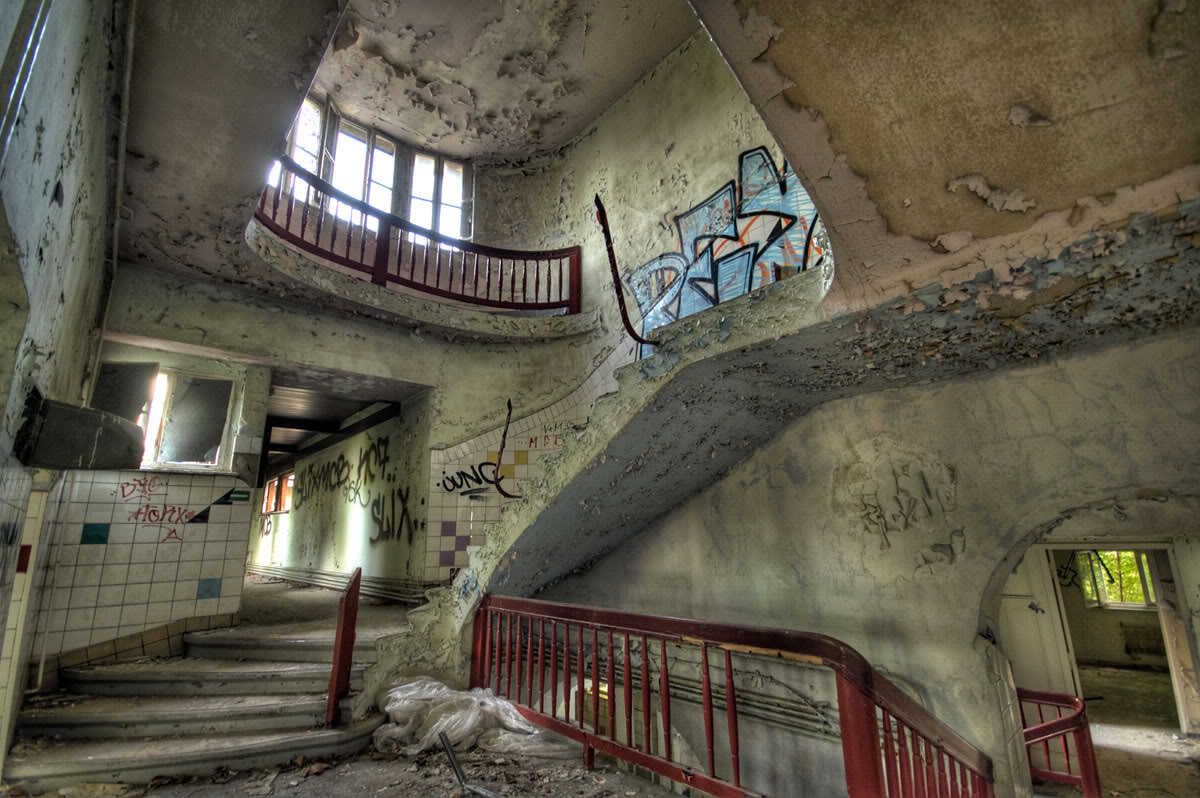
\includegraphics[scale=0.2]{scp/026a.jpg}
\linebreak Main foyer of SCP-026
\end{center}
\end{figure}

\textbf{Special Containment Procedures:} SCP-026 is to remain securely locked and boarded up at all times when there is no research ongoing. Alarms are set to alert the Foundation in case of entry by civilians or other agencies.

\textbf{Description:} SCP-026 is a three (3) story public school building built in \censor{XXXX}. It has two (2) wings connected to a central foyer. It was declared condemned in \censor{XXXX} after it was found the floor plan didn't match up to the building's blueprints (see Interview Log 026-01). It came to the Foundation's attention after several disappearances in the area were linked to visits to the abandoned building.

\sout{The building demonstrates spatial anomalies. Its internal space is much greater than the external surface of the building would allow. Hallways display variable length, while stairways have differing numbers of steps going up or down. The number of rooms off of the hallways changes each time they are counted. Attempts to reach the far ends of the hallways have met with failure thus far. Entrance through the fire escapes located at the ends of the hallways leads to doors approximately midway down the length of the halls.}

\textbf{EDIT:} See Note 026-A

\begin{figure}[h]
\begin{center}
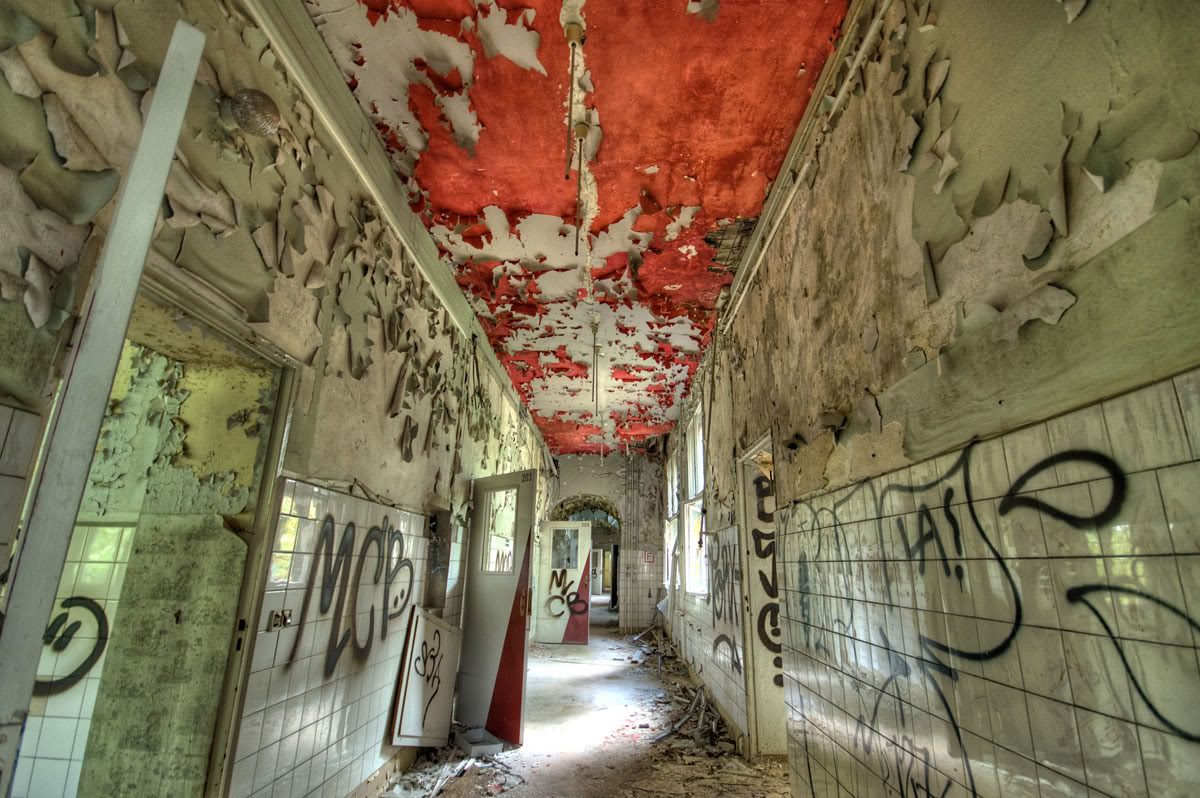
\includegraphics[scale=0.2]{scp/026b.jpg}
\linebreak Second floor hallway of the east wing
\end{center}
\end{figure}

There is considerable graffiti on the interior walls of the school. Most appears typical, including gang signs, names, and street art. However, the graffiti fades and reappears, changing location. Writing on chalkboards and bulletin boards changes in a similar fashion. Subjects typically found range from standard school subjects (mathematics, literature, biology), to more esoteric subjects, such as quantum entanglement, \censor{XXXXXXXX}, and eugenics. One researcher reported one board detailing information about SCP-\censor{XXXX}, but photographic evidence showed only a blank slate (See Note 026-B). The phrase "The children used to sing" has appeared multiple times in various places throughout the building, but there is currently no explanation for its significance.

A number of unconscious subjects have been found in the building, mostly of high school age, ranging from twelve to eighteen. They are dressed in accordance to the school's dress code, circa \censor{XXXX}. Several have been identified as former students or faculty of the school who disappeared after the school shut down (in at least one case, more than ten years after the closure). It is currently unknown how they were transported back into SCP-026. (See Note 026-C)

\begin{figure}[h]
\begin{center}
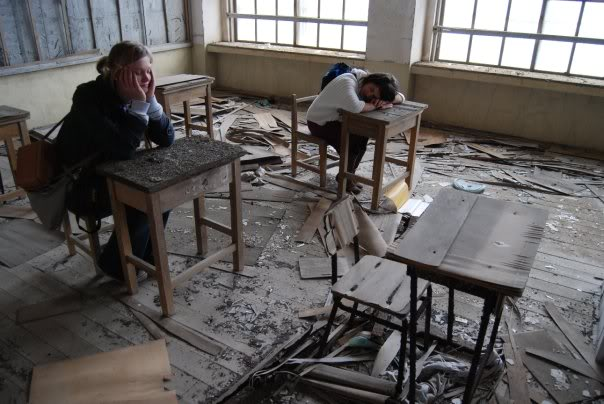
\includegraphics[scale=0.4]{scp/026c.jpg}
\linebreak Subjects discovered within SCP-026
\end{center}
\end{figure}

All attempts to wake the subjects while inside the building have failed. On being removed from the grounds of SCP-026, the subjects wake abruptly. They experience a period of confusion, before dying from extremely rapid dehydration, followed by advanced decomposition. No useful intelligence has been recovered from the subjects to date.

The inability to wake subjects extends to those who fall asleep on the grounds of SCP-026, though the rapid dehydration only seems to affect those who have been found on the grounds of the school. See Incident Report 026-12.

\textbf{Note 026-A:} Robotic exploration and video feeds have shown that the apparent spatial anomalies are caused by changes in the perceptions of observers, rather than actual spatial phenomena. For this reason, SCP-026 does not require the expertise of Mobile Task Force Rho-8 "Roadside Picnickers" at this time.

UPDATE: Further exploration has shown that some spatial phenomena do occur. See the Exploration Logs for more details.

\textbf{Note 026-B:} The contents of notepads, books, and pieces of paper have been observed to disappear, only to reappear on surfaces within SCP-026. New writings have appeared, mostly drawn from graffiti or text-books. Caution should be exercised in bringing documents onto the grounds of SCP-026.

\textbf{Note 026-C:} Several class D personnel exposed to SCP-026 have disappeared from Foundation control, only to reappear inside the anomalous building. The subjects in question had previously complained of dreams identical to those experienced by Agent Malek.

UPDATE: See Interview Log 026-08.

\textbf{Incident Report 026-12}
During a routine security check of SCP-026, Agent Malek was found unconscious by his partner, Agent Jones, in the main foyer. Initial attempts at rousing Agent Malek were ineffective, so he was moved for transportation to Site \censor{XX}. Upon leaving the grounds of SCP-026, he woke abruptly in a state of agitation. When questioned, he revealed that he had been dreaming of a classroom setting. This dream has been consistent throughout all subjects who have fallen asleep within the grounds of SCP-026.